\section{Training for ‘Unstable’ CNN accelerator} \label{sec:framework}
  In contrast to the conventional off-line training on CPUs and GPUs, we propose 
to take these accelerators’ dynamic behaviors into consideration during training 
to tolerate the ‘un-deterministic’ behavior of the ‘unstable’ accelerators. The basic 
idea is to embed the CNN accelerator into the conventional training framework so that 
the accelerator is referenced during training. In this work, we choose Caffe as the baseline 
training framework because it is more natural to integrate the C/C++ based high 
level synthesis CNN accelerator. Based on Caffe, we further detail the required general 
interface to make use of the hardware accelerator in training, and introduce 
the necessary modifications to the CNN accelerator structure. 
\subsection{Proposed Training Framework }
  Figure 3 illustrates the proposed training framework. It begins with the 
off-line training result which can greatly shorten the overall training time. 
While most of the CNN accelerator adopts fixed point operations, the pre-trained model 
is therefore expected to be fixed point model. With the pre-trained model, 
we mainly try to have the trained model to further adapt to the ‘un-deterministic’ 
behaviors which are difficult to model on CPUs and GPUs.

\begin{figure*}
        \center{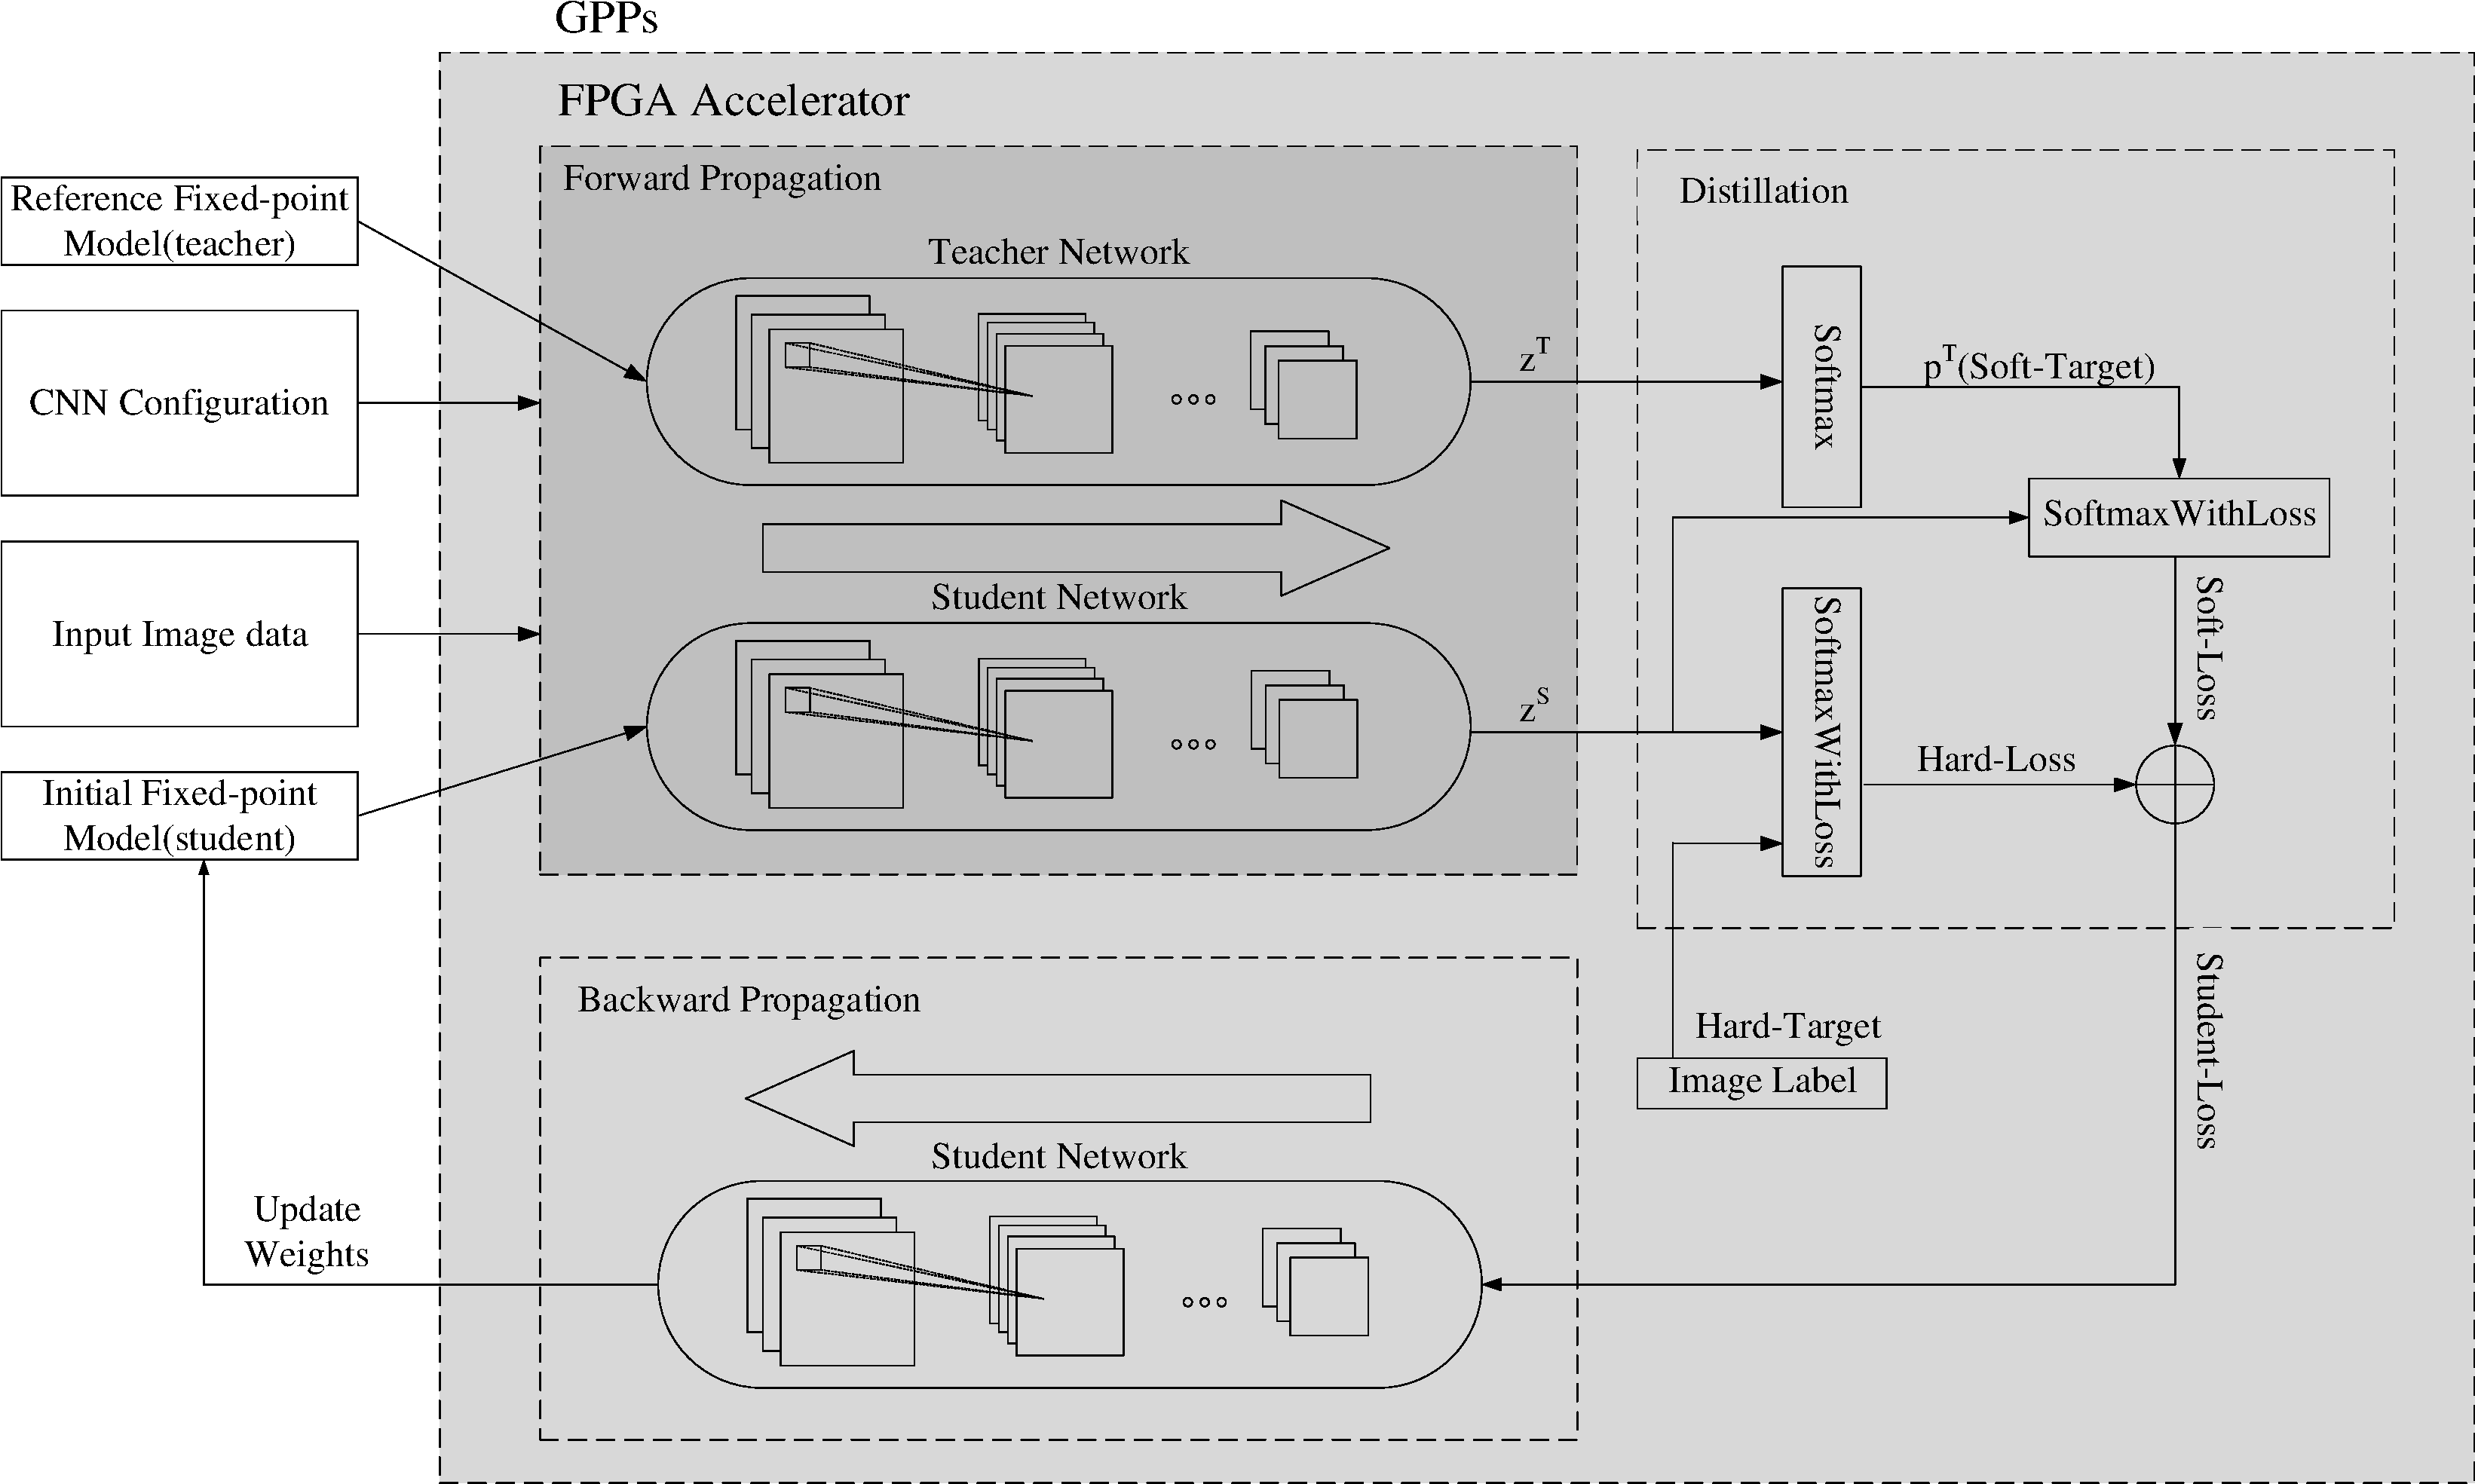
\includegraphics[width=0.85\linewidth]{retrain}}
        \caption{Training Framework}
        \label{fig:retrain}
%        \vspace{-0.5em}
\end{figure*}


  To that end, we have the forward propagation performed on the accelerator 
directly while the backward propagation remains on CPUs or GPUs. Forward propagation 
on the accelerator is fixed point, which is beneficial to both the resource consumption 
and memory bandwidth overhead, but backward propagation on CPUs or GPUs remains floating 
point to ensure the small changes in the parameters get accumulated\cite{Matthieu2014_8}. As a result, 
we still need additional converting between the fixed point and floating during 
the training in each iteration when the weight is adjusted. When the final accuracy 
loss reaches the threshold, it means that the model can tolerate 
the accelerator’s ‘un-deterministic’ behaviors. And the CNN model can be safely 
deployed on the ‘unstable’ accelerator. 

Figure 4 depicts the implementation of the training framework on a hybrid 
CPU-FPGA architecture. In this work, we use Xilinx KCU1500 as the FPGA board 
and put it on a standard desktop computer. CPU is the controller and it reconfigures 
the accelerator for a specific CNN structure. In each training iteration, CPU launches 
the CNN accelerator to perform the forward propagation from bottom layer to top layer. 
CPU does the backward propagation from top layer to bottom layer. Weights and the image 
data are initially stored in host memory. It will be transferred to FPGA offchip memory 
for forward propagation through PCI-E. Similarly, the output data will be transferred 
from FPGA off-chip memory back to host memory after forward propagation. Because of the 
OpenCL based API wrapper in SDAccel, the CNN accelerator’s interface can be easily 
exposed to Caffe for referring to the forward propagation result. 

%\begin{figure}
%        \center{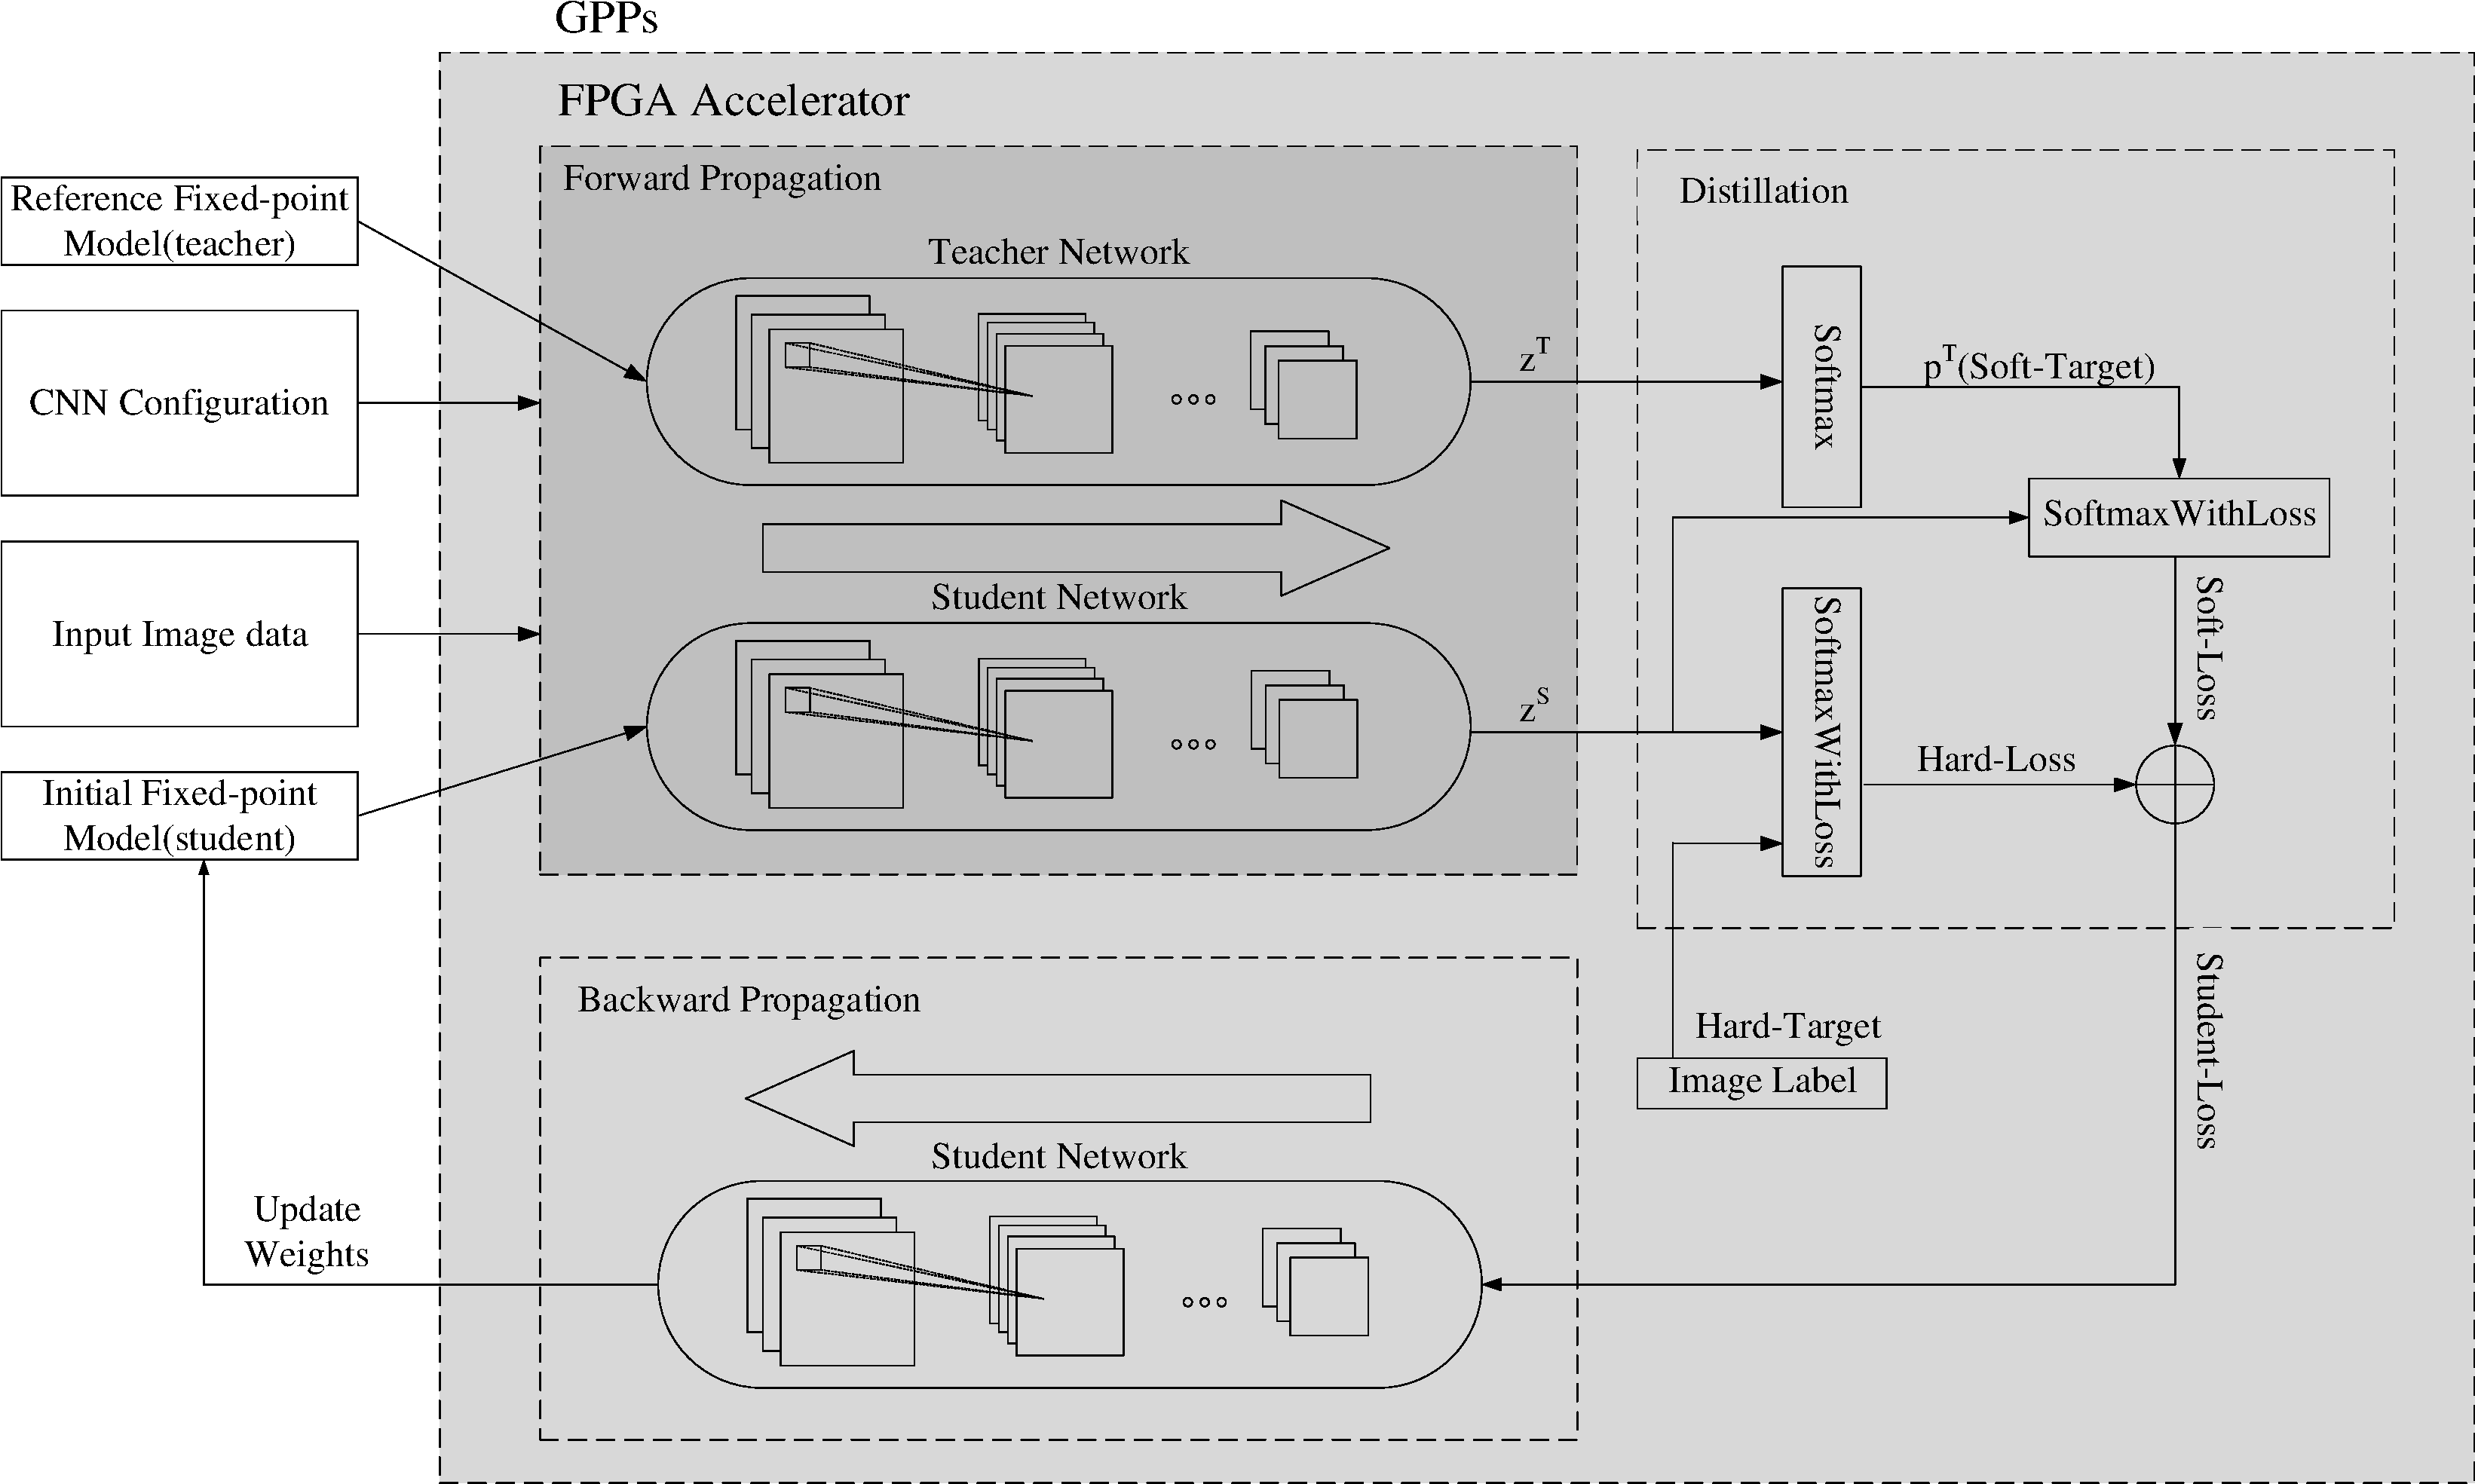
\includegraphics[width=0.85\linewidth]{retrain}}
%        \caption{Training on Hybrid CPU-FPGA Architecture}
%        \label{fig:framework}
%        \vspace{-1em}
%\end{figure}


\subsection{High Level Accelerator Interface to Caffe }
  With the growing popularity of deep learning, massive different 
CNN accelerators have been developed over the years. In order to fit various CNN accelerators 
within the same training framework, we define a set of high-level interface functions as listed 
in Table 1. There are 7 functions included. Function 1 is used to launch the CNN accelerator from host. 
Function 2 and 3 are used to transfer data between the host memory and the device memory during 
the training. As most of the accelerators are fixed point and used for forward while back propagation 
is floating point, Function 4 and 5 are required for training when forward and backward 
propagation are iteratively committed. Function 1 to 5 are required for all the accelerators. 
Function 6 and 7 are only needed for accelerators that perform on reorganized data\cite{pipecnn_2,deepburing_12}. 
With the interface functions, general CNN accelerators can be trained to tolerate ‘un-deterministic’ circuit 
behaviors using the proposed framework.
  CNN accelerators can either be implemented using high-level synthesis tools (HLS) or hardware description 
languages (HDL). With Xilinx SDAccel, we can wrap the both types of accelerators with OpenCL API. 
With the OpenCL API, Caffe can refer to the accelerators during training conveniently. 

\begin{table*}
        \centering
        \vspace{-0.3em}
        \caption{High-level interface to integrate general CNN accelerators with Caffe}
        \label{tab:graph}
        \vspace{-0.3em}
        \begin{tabular}{c|l|l}
                \toprule
                ID & Function Name & Description  \\
                \midrule
                1 & launchAccelerator() & It configures the CNN accelerator and launches it from host CPU. \\
		\midrule
                2 & dataToFPGA(weight, input, wgtDevAddr, inDevAddr) & It transfers both the input data and weight to the FPGA device memory. \\
		\midrule
		3 & dataFromFPGA(outputDevAddr, output) & \shortstack[l]{It transfers all the intermediate output of the CNN layers from FPGA \\device memory to host memory.} \\
		\midrule
		4 & convertIntToFloat(int iData, float fData) & It converts the fixed-point output to float for back propagation processing. \\
		\midrule
		5 & convertFloatToInt(float fData,  int iData) & \shortstack[l]{It converts the floating-point input and weight data to fixed point or \\integer for forward processing on the accelerator.} \\
		\midrule
		6 & dataLayoutReorder(data, reorderedData) & \shortstack[l]{It reorders the data layout for more efficient accelerator execution before \\sending to FPGA device memory.} \\
		\midrule
		7 & dataLayoutRecover(reorderedData, data) & It reorders the output data back to the default format for Caffe back propagation. \\
                \bottomrule
        \end{tabular}
        \vspace{-1em}
\end{table*}

\subsection{Modification to the general CNN accelerators}
  On top of the interface, the CNN accelerator also needs minor adjustment for the training. 
The training process requires the feature maps of each CNN layer for backward propagation, 
while the accelerators are typically optimized for inference and some of the layers’ output 
are fully buffered in on-chip memory for less memory access overhead. In this case, 
the accelerator should make intermediate output write back optional as shown in Figure 5. 
When the accelerator is used in training, the output will be transferred to memory. 
When it is used for inference, it can also turn off the write back data path for better performance. 
It is trivial to modify the CNN accelerators and the hardware overhead is negligible.

\begin{figure}
        \center{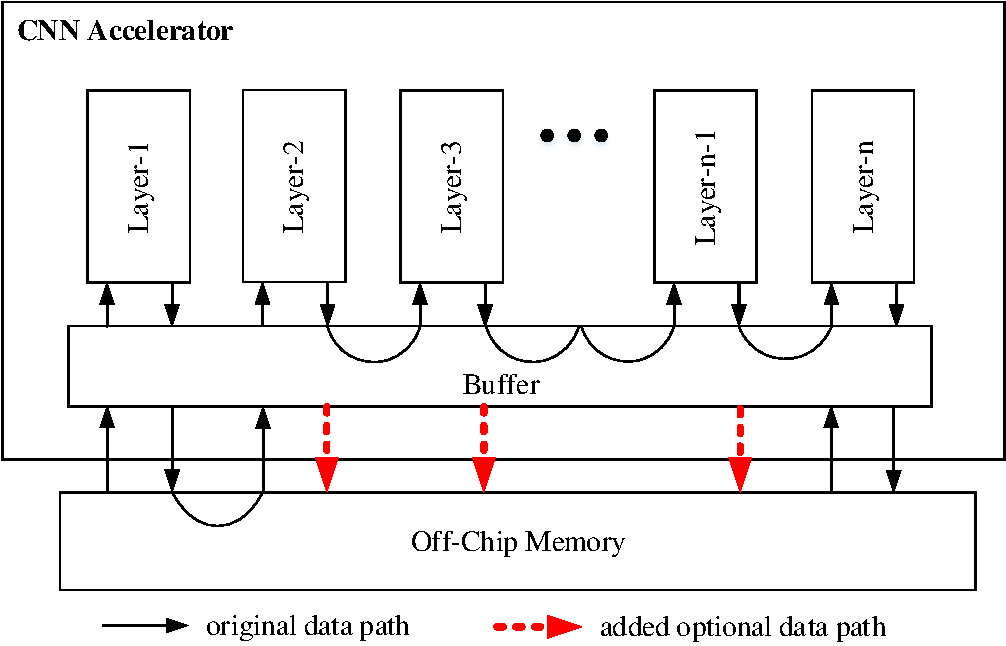
\includegraphics[width=0.85\linewidth]{change_of_accelerator}}
        \caption{Modification of the CNN accelerator data path. It essentially
ensures each CNN layer to have an optional data path to off-chip memory so that it
can be used for training as necessary.}
        \label{fig:change_of_accelerator}
        \vspace{-1em}
\end{figure}

\section{Case Study and Experiments} \label{sec:casestudy}
  In this section, we mainly explore deploying the CNN models on the ‘unstable’ accelerators 
using the proposed training framework. In particular, we take an overclocked CNN accelerator 
and a soft error attacked CNN accelerator as typical ‘unstable’ accelerator examples.

  Four convolution neural networks including LeNet, AlexNet, VGG-16 and VGG-19 are used.
They are implemented on Xilinx KCU1500 based on 8bit fixed-point PipeCNN using SDAccel 2017.1. 
The FPGA cards is attached to a desktop computer configured with Intel(R) Core(TM) i7-2600 
CPU (4core, 3.40GHz) via PCI-e 2.0. The communication bandwidth is 8GB/s.

\subsection{Overclocked CNN accelerator}
  Clock frequency is almost proportional to the computation capability of the CNN accelerator 
when its architecture is determined. While timing analysis tools typically recommend a 
conservative clock frequency in order to avoid the possibility of timing violations, 
FPGA designs can be safely overclocked by a significant ratio with respect to the maximum 
operating frequency estimated by the FPGA’s tool flow. This gives the advantage of increasing 
the implementation throughput without any design-level modifications. Beyond this safe overclocking 
margin, some critical paths in the design starts to fail and the output error rate increases 
exponentially with respect to the increase in the clock frequency. To tolerate the computing 
error and gain the performance benefit, we thus opt to use the proposed training framework.  

  With PipeCNN, we implemented four CNN including LeNet, AlexNet, VGG-16 and VGG-19 on KCU1500. 
As PipeCNN provides customized implementation for different CNN, the baseline frequency of the implementations 
is different. The frequency of the four implementations is 210Mhz, 210MHz, 190MHz and 190MHz respectively. 
Then we boost the clock frequency gradually and train for the ‘unstable’ CNN accelerator implementations on 
ImageNet data set.  The prediction accuracy of the resulting implementations is presented in Figure 6. In general, 
overclocking can enhance the clock frequency by 19\% to 26\%. While applying the off-line trained model 
to the accelerator with overclocking, the top-5 accuracy degrades by up to 4.3\%. When the proposed training 
framework is used, the resulting retrained model can be much better especially near the overclocking limit.

  For AlexNet, VGG-16 and VGG-19, the top-5 accuracy of the retained models is improved by 3.4\%, 1.8\%, and 2\% 
respectively at the extreme overclocking frequency. For LeNet which is a rather small yet reliable network 
compared to the other three, the implementation remains unaffected even when the clock is boosted to 260 MHz 
from 210 MHz. When the clock goes up to 270MHz, the timing error can no longer be tolerated by the hardware system, 
the prediction accuracy drops to 10\% which is essentially meaningless. In this case, the base model 
and the retrained model is pretty much the same. To ensure the stability of the overclocking experiment, 
we also keep measuring the accuracy of the accelerators with extreme overclocking. With repeatedly 
running the test for up to 40 hours, the measured accuracy varies slightly as present in Figure 7. 
Despite the fact that the errors caused by the overclocking can be hardly modeled precisely at runtime, 
the inherent error patterns may still partly be captured by the CNN model with the proposed training. 
This explains the higher prediction accuracy with the retrained model. According to the 
above experiments, we can conclude that the proposed accelerator aware training can produce 
more resilient CNN model tolerating errors caused by intensive overclocking. 

\begin{figure}
        \center
	\subfloat[]{
		\label{fig:lenet}
		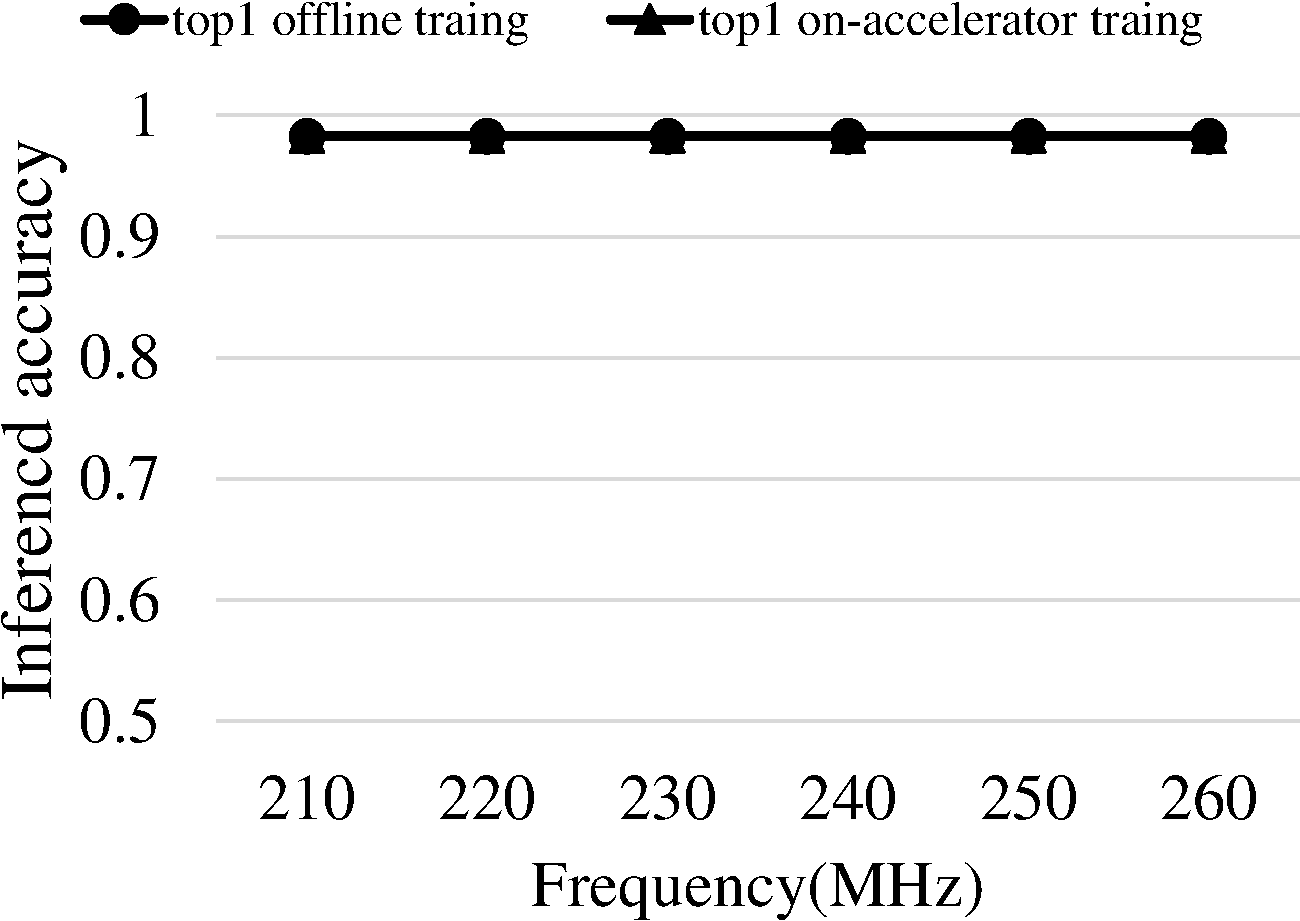
\includegraphics[width=0.4\linewidth]{lenet-overclock}
	}
	\qquad
	\subfloat[]{
                \label{fig:alexnet}
                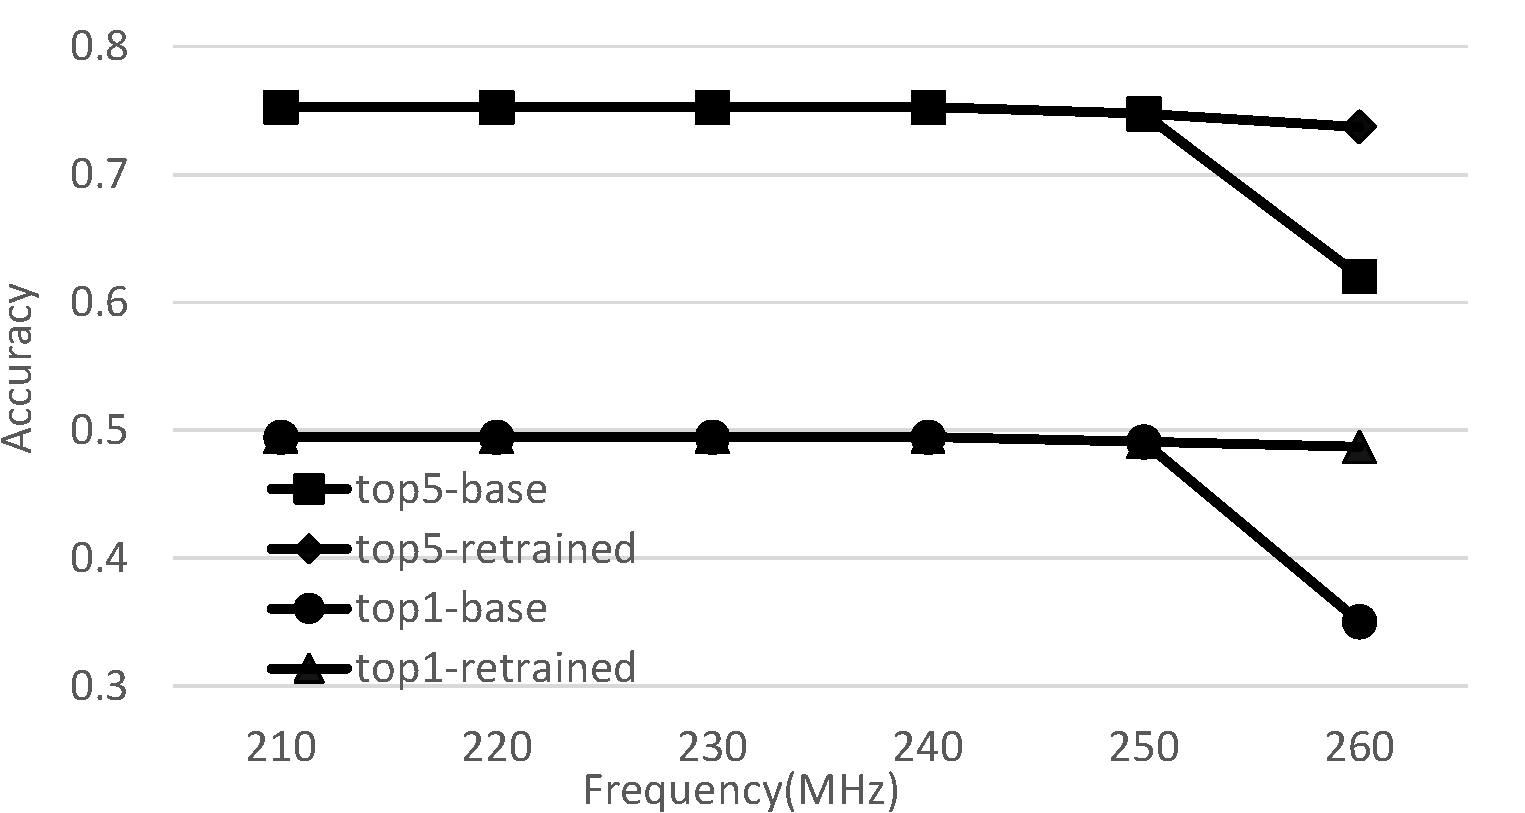
\includegraphics[width=0.4\linewidth]{alexnet-overclock}
        }
	\qquad
	\subfloat[]{
                \label{fig:vgg16}
                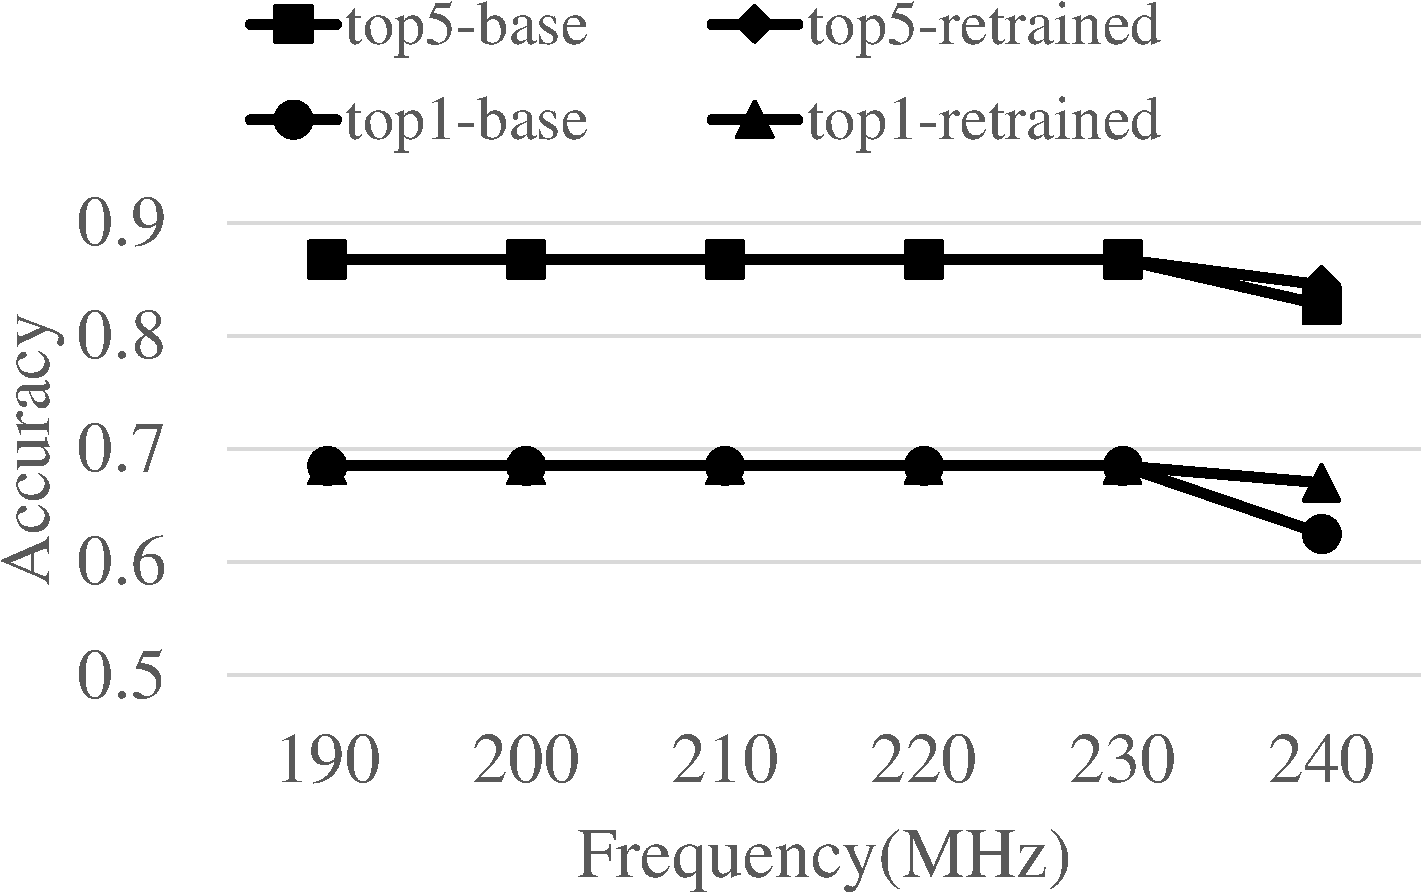
\includegraphics[width=0.4\linewidth]{vgg16-overclock}
        }
        \qquad
	\subfloat[]{
                \label{fig:vgg19}
                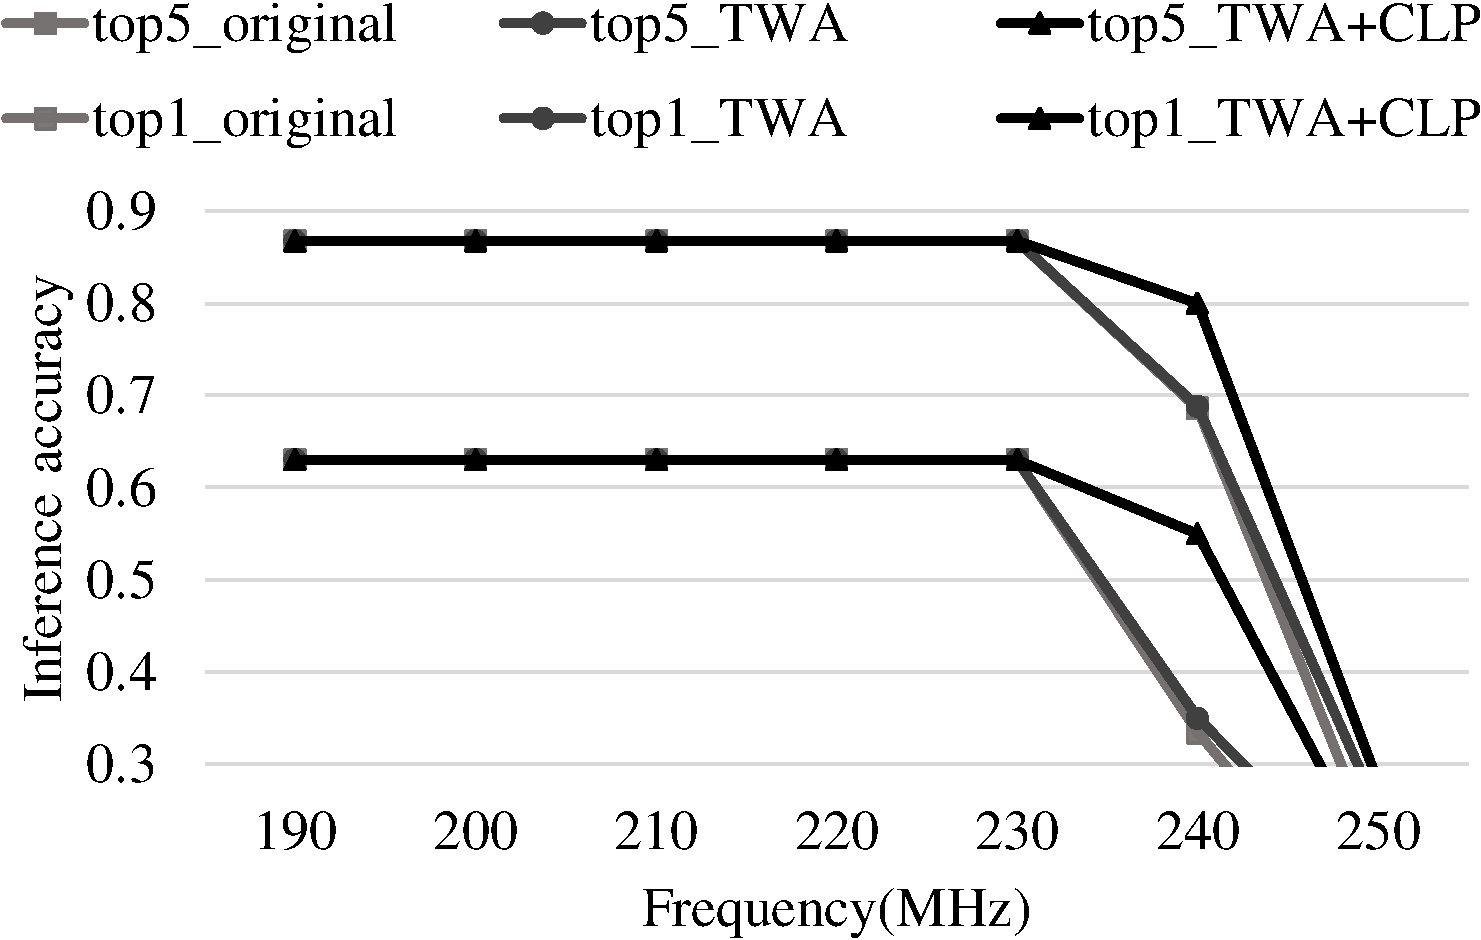
\includegraphics[width=0.4\linewidth]{vgg19-overclock}
        }
	\caption{The Accuracy of Four CNN models on accelerators with different overclocking frequency}
        \label{fig:overclock accuracy}
\end{figure}

To ensure the stability of the overclocking experiment, we 
also keep measuring the accuracy of the accelerators with extreme 
overclocking. With repeatedly running the test for up to 40 hours, 
the measured accuracy varies slightly as present in Figure 7. 
Despite the fact that the errors caused by the overclocking can be 
hardly modeled precisely at runtime, the inherent error patterns may 
still partly be captured by the CNN model with the proposed training. 
This explains the higher prediction accuracy with the retrained model. 
According to the above experiments, we can conclude that the proposed 
accelerator aware training can produce more resilient CNN model tolerating 
errors caused by intensive overclocking. 

\begin{figure}
        \center{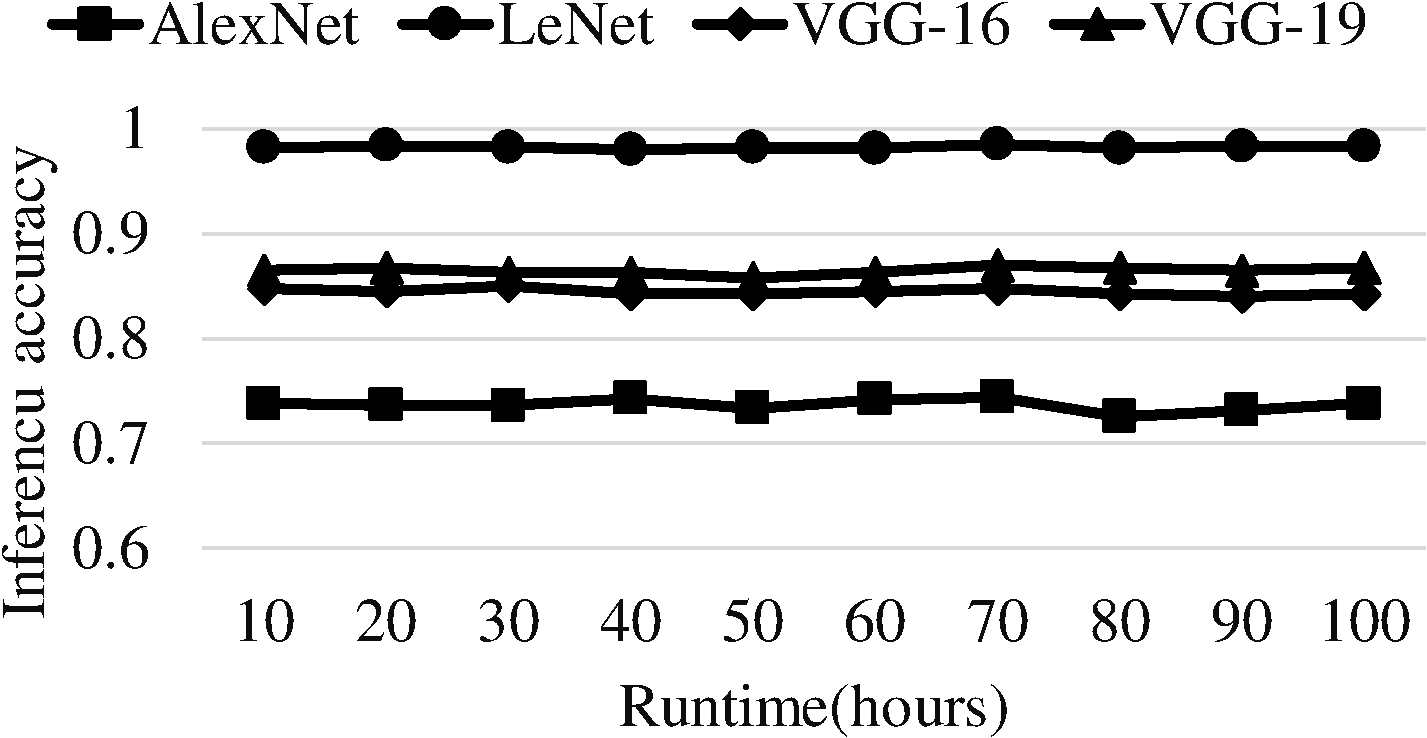
\includegraphics[width=0.85\linewidth]{stability}}
        \caption{The Stability of Retrained Model}
        \label{fig:stability}
%        \vspace{-0.5em}
\end{figure}

  Finally, we also present the training time on the hybrid CPUFPGA architecture. 
It can be seen that the training is much slower than the fixed-point training on CPU. 
This is mainly caused by the frequently data transferring between device memory and host 
memory in the proposed training, while this will not affect the inference time. In addition, 
we can also find that the training on larger network takes longer time and higher clock frequency 
is also beneficial to the training time as expected. 

\begin{figure}
        \center{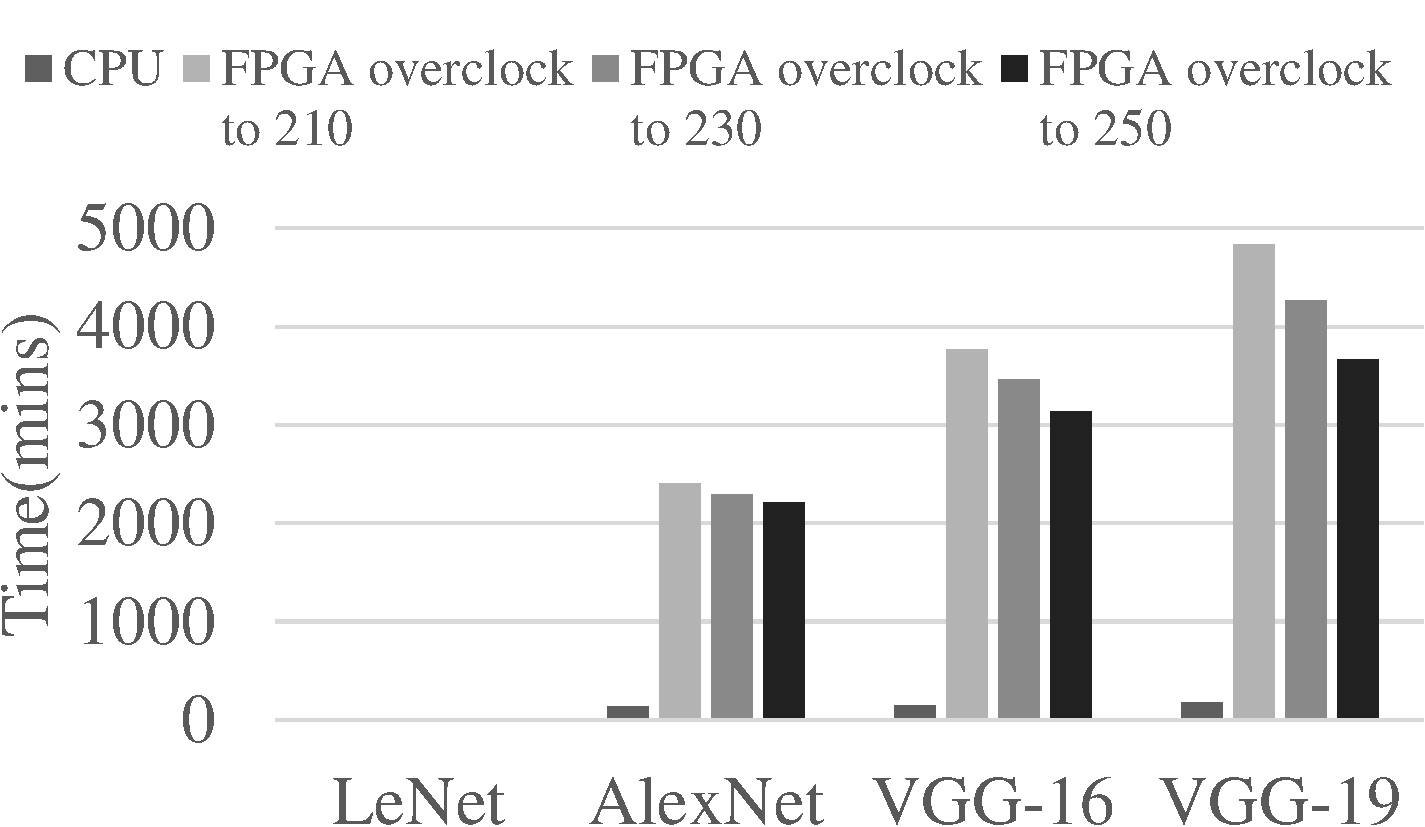
\includegraphics[width=0.85\linewidth]{time}}
        \caption{Training time}
        \label{fig:time}
%        \vspace{-0.5em}
\end{figure}


\subsection{CNN accelerator with soft errors}
  With the shrinking semiconductor feature size and increasing FPGA capacity, 
FPGA design gets error-prone to the transient faults (often known as soft errors). 
They can affect the behaviors of the FPGA design dramatically. Many researchers \cite{Mansour_20,Karim_21,Nidhin_22,Subasi_23,ROSCH_24} 
have proposed diverse approaches to address this problem. While CNN accelerators on FPGA can be different 
from general hardware design because the CNN model deployed can be further trained and tolerate the 
soft errors as proposed in prior section\cite{Tu2018RANA_1}.

  To explore the influence of soft errors on CNN accelerator, we need to inject soft errors to the system first. 
A number of fault injection techniques have been proposed in prior literature. In this work, we adopt 
a simple software simulation- based method to inject random errors. Although the error may be caused by 
on-chip memory or other SRAM cells, we have a random bit of the computing result flipped at a specific rate. 
The simple yet representative model will not increase the training time too much.

  We also take LeNet, AlexNet, VGG-16, and VGG-19 to evaluate the influence of soft errors on prediction accuracy,
the top-5 accuracy of the resulting implementations is presented in Figure 9. When we gradually 
increase the error rate from 1E-7 to 1E-5, the prediction accuracy degrades accordingly when applying the off-line 
trained model directly on the faulty accelerator. When the error rate goes up to 1E-4.5, 
the accuracy in the worst case drops by around 13.5\%. Similar to overclocking, LeNet can tolerate 
more errors than the other three networks. The accuracy remains unchanged until the error rate reaches 1E-3. 
When the error injection rate is low, the CNN model is able to cover almost all the negative influence 
on the prediction accuracy.

\begin{figure}
        \center
        \subfloat[]{
                \label{fig:lenet}
                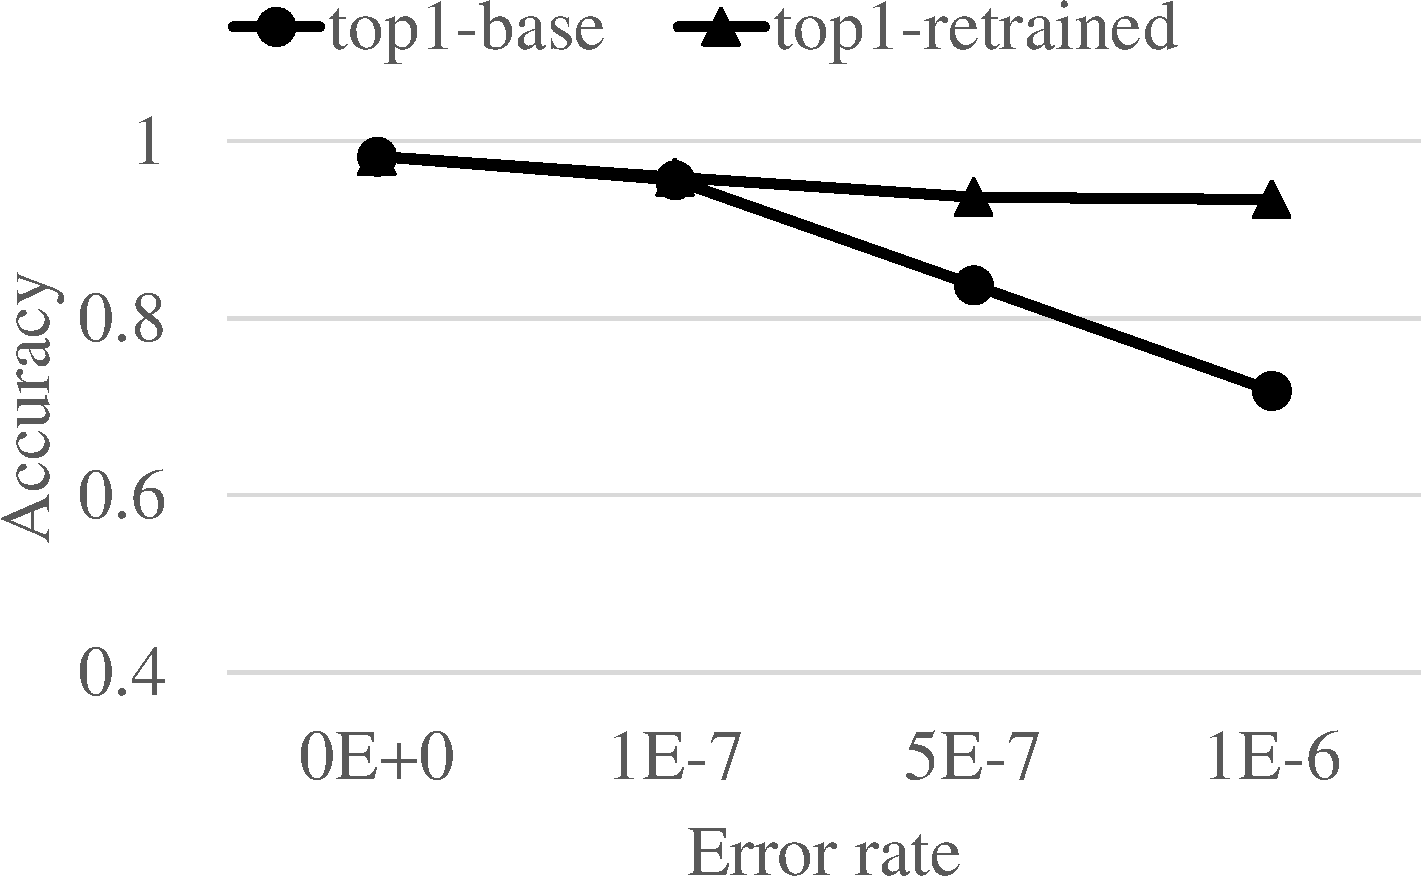
\includegraphics[width=0.4\linewidth]{lenet-softerror}
        }
        \qquad
        \subfloat[]{
                \label{fig:alexnet}
                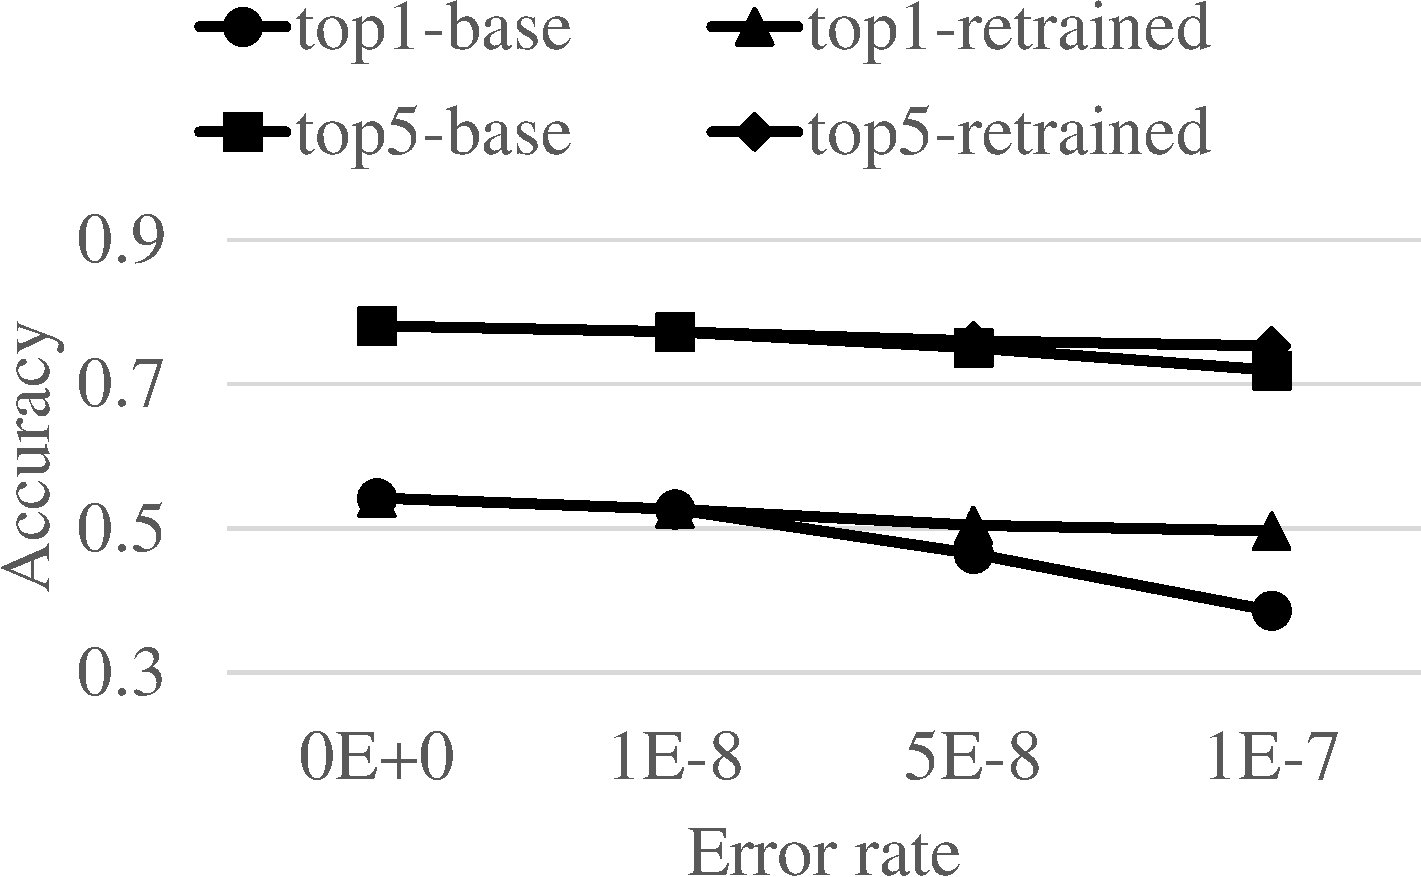
\includegraphics[width=0.4\linewidth]{alexnet-softerror}
        }
        \qquad
        \subfloat[]{
                \label{fig:vgg16}
                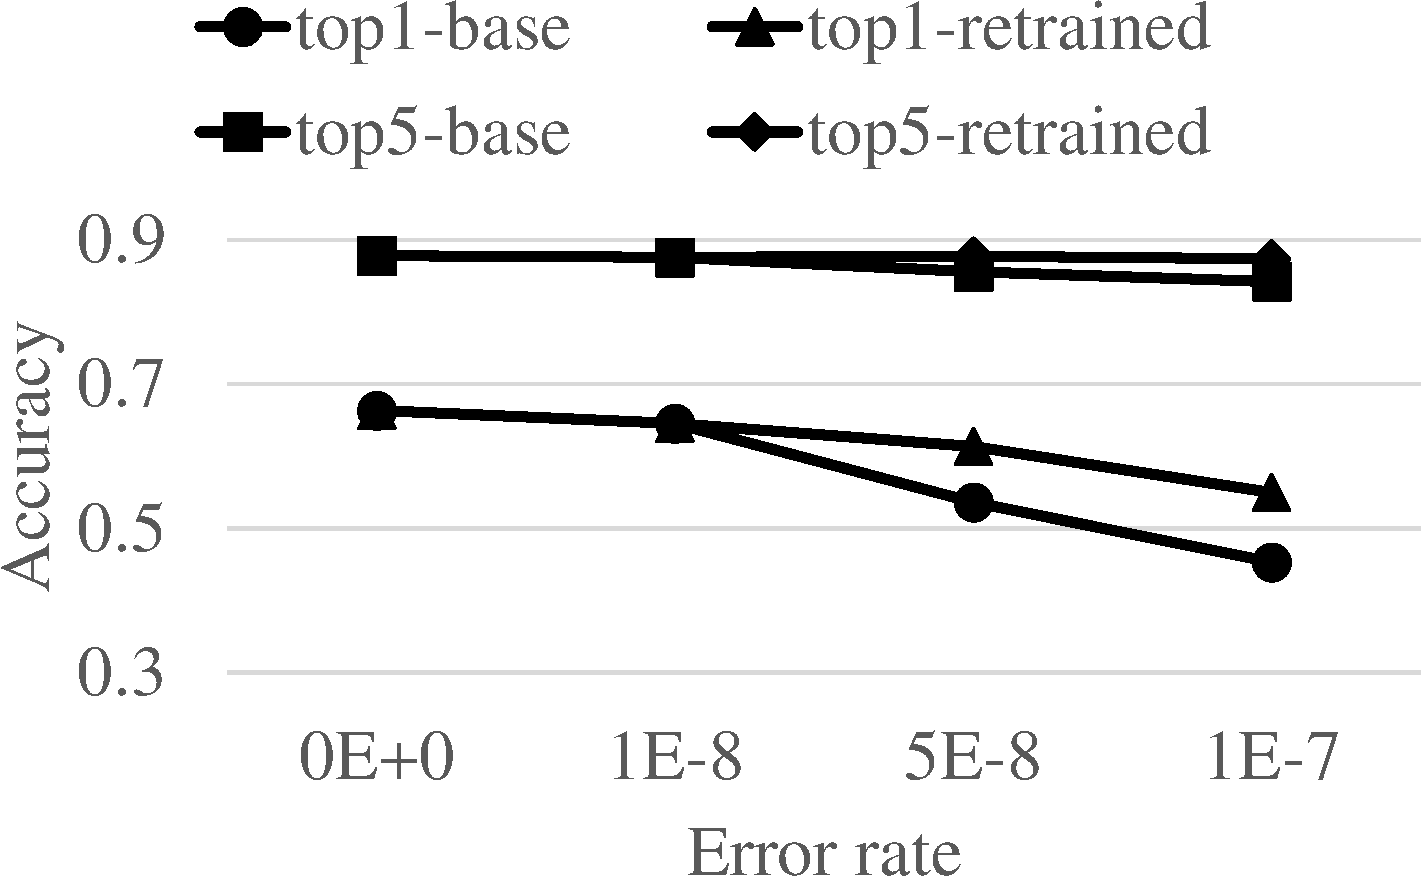
\includegraphics[width=0.4\linewidth]{vgg16-softerror}
        }
        \qquad
        \subfloat[]{
                \label{fig:vgg19}
                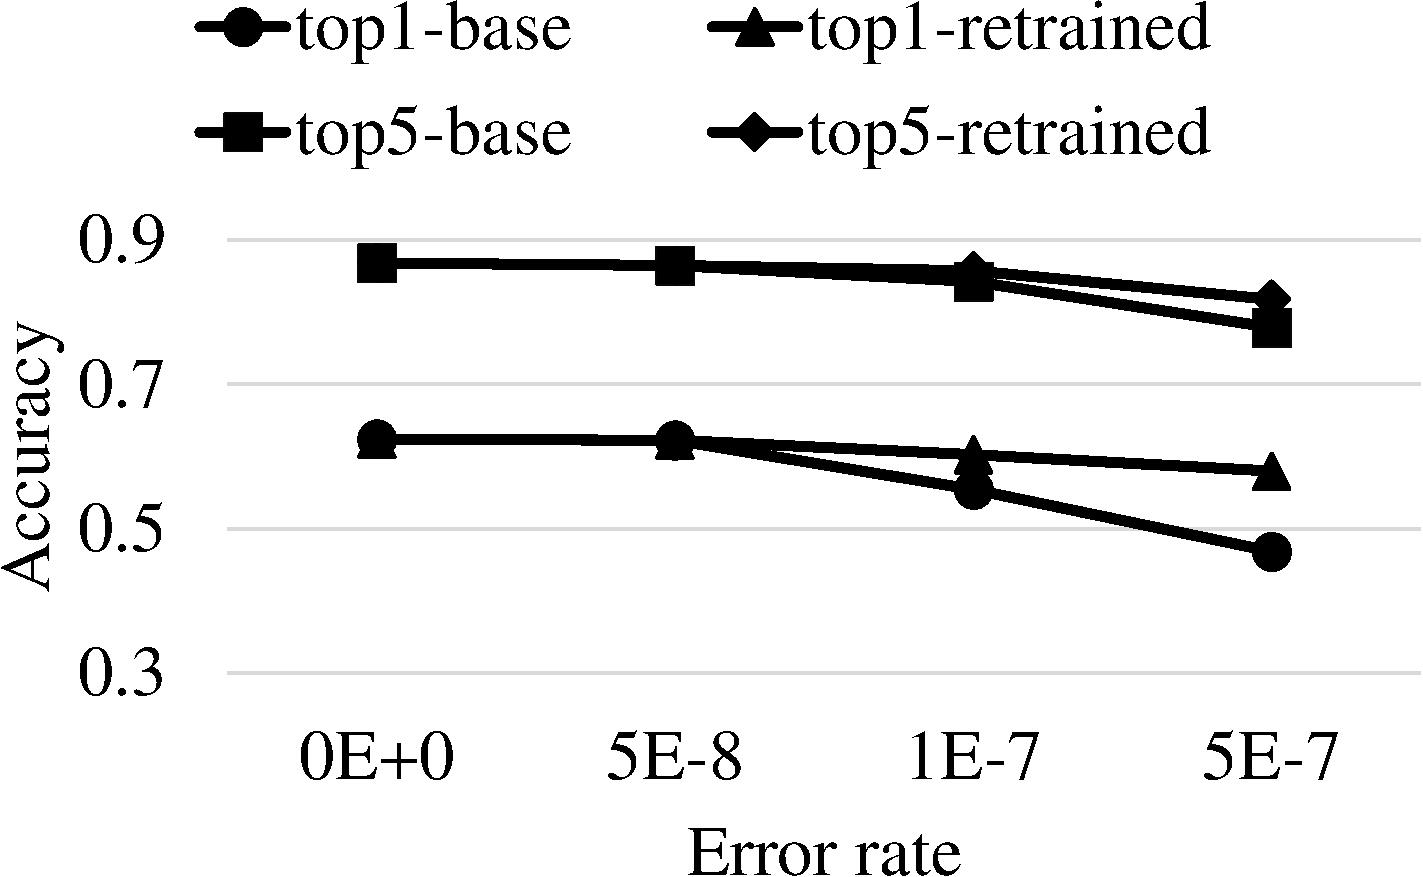
\includegraphics[width=0.4\linewidth]{vgg19-softerror}
        }
        \caption{The Precision of Four CNN models on accelerators with different error rate}
        \label{fig:softerror accuracy}
\end{figure}


  When the error injection rate goes higher, the proposed retraining becomes critical. 
According to the experiments, the accuracy of the four retrained models improve by 6.8\%, 1.5\%, 3\%, and 3\% 
respectively compared to that of the base model when the accelerators are exposed to the highest 
error injection. In summary, the experiments demonstrate that we can have the CNN model to learn 
both the characteristics of the data and the underlying ‘undeterministic’ behaviors of the accelerator 
together using the proposed training framework. The resulting CNN model can improve the accuracy 
without any modification on the accelerator when there is high error injection rate.  

\section{Related Work} \label{sec:relatedwork}
\textbf{CNN accelerator:} There have been notable efforts made to create hardware accelerators of 
machine learning algorithms for the sake of higher performance and energy-efficiency \cite{Cnvlutin_25} 
in the past few years. Among the accelerators, the regular 2D array architecture has become 
a mainstream solution because of the relatively higher PE and bandwidth utility. Runtime reconfigurable 
PE arrays are applied to provide customized solutions for efficient CNN inference on FPGAs \cite{Caffeine_6,deepburing_12}. 
In \cite{Aydonat_27}, an array of processing elements (PEs) with novel architecture was developed. With intensive 
data reuse, it reduces the external memory bandwidth requirements dramatically and outperforms 
the systolic-like structure proposed in \cite{Caffeine_6}. Compared to the compact hardware design in \cite{Caffeine_6,Aydonat_27}, 
Wei X et al. in \cite{Wei_29} implemented a high-throughput CNN design and did comprehensive design space exploration 
on top of accurate models to determine the optimal design configuration.

\textbf{Training of accelerators:} Training approaches for CNN accelerator can be classified into three 
categories: (1) convert a pretrained floating point CNN model into a fixed point model without 
training, (2) train a CNN model with fixed point constraint, and (3) FPGA-implemented forward \& backward propagation 
training tools. For first category, \cite{Yunchao_19} applied codebook based on scalar and vector quantization methods 
in order to reduce the model size. \cite{Cnvlutin_25} analyzed the quantization sensitivity of the network for each layer 
and then manually decide the quantization bit-widths. \cite{Hwang2014_17} find direct quantization for fixed-point 
network design does not yield good results and optimized the fixed-point design by employing back propagation 
based retraining. \cite{Matthieu2014_8} adapted a higher precision for the parameters during the updates than during 
the forward and backward propagations for accumulating small changes in the parameters. \cite{Hwang2014_17} used only binary 
weights to train deep neural networks. 

  However, these approaches of the former two categories are not suitable for ‘unstable’ circuit. 
For the third category, FCNN\cite{fcnn_5}  reconfigured a streaming data path at runtime to cover the training cycle 
for the various layers in a CNN. Caffeine\cite{Caffeine_6}  provides tunable parameters, including the number and 
size of input/output feature maps, shape and strides of weight kernels, pooling size and stride, 
ReLU kernels, and the total number of CNN/DNN layers. Caffeinated FPGA\cite{DiCecco_4} implemented FPGA kernels 
for forward and backward for Caffe and these kernels target the Xilinx SDAccel OpenCL environment 
for training and inference with CNNs. However, these approaches did not consider the unstable 
hardware behavior into their framework or either gave a way to train CNN under the un-deterministic situation.

\textbf{Unstable Hardware Behavior:} Overclocking, soft Error, circuit defect induced by process 
variation etc. result in the un-determined behavior of the circuits.  Overclocking, a technique to gain 
the additional performance from a given component by increasing its operating speed, may cause timing error. \cite{overclock_3} gave 
the strands of research of arithmetic precision determination and overclocking. Razor\cite{Razor_15}  projected scaled 
the supply voltage and clock frequency beyond the most conservative value. Soft errors are unintended 
transitions of logic state in a circuit typically caused external source of ionizing radiations. 
The shrinking transistor sizes increased the soft-errors. \cite{Mansour_20} proposed An Automated SEU 
Fault-Injection Method and Tool for HDL-Based Design. \cite{Subasi_30} inject single-bit flips into the register-transfer 
level descriptions of floating-point ALUs.

\section{Conclusion} \label{sec:Conclusion}
In this paper, we propose to take the CNN accelerator’s ‘undeterministic’ behaviors into consideration 
at training and have the CNN model to learn the accelerator’s behaviors. To that end, we further build 
an open-sourced training system based on Caffe on a hybrid CPU-FPGA architecture. Then use the training 
system to deal with an overclocked CNN accelerator and an accelerator with soft errors. According to our 
experiments, the proposed training can improve the prediction accuracy of four CNN models up to 3.4\% when 
the CNN accelerator is overclocked on the extreme situation. This method is also beneficial to the CNN 
accelerators with soft errors. In the case with most soft errors, it improves the prediction accuracy up 
to 6.8\% and by 3.58\% on average. The disadvantage is the much longer training time due to the frequent 
data transfer between host memory and device memory. This problem can be resolved when porting the system 
to closely coupled CPU-FPGA architectures with shared memory.

%\appendix
%\section{Acknowledgement}

%\begin{acks}
%  The authors would like to thank Sam Ho for providing the suggestions on
%  HLS design debugging and optimization as well as the SDAccel usage. 

%\end{acks}
